\documentclass[pdflatex,sn-mathphys-num]{sn-jnl}
\usepackage{amsmath,amssymb,amsfonts}
\usepackage{algorithmic}
\usepackage{graphicx}
\usepackage{tikz}
\usetikzlibrary{shapes,arrows}
\usepackage{textcomp}
\usepackage{xcolor}
\usepackage{booktabs}
\usepackage{tabularx}
\usepackage[T1]{fontenc}
\usepackage{array}
\usepackage{float}
\usepackage{url}
\usepackage{multirow}
\usepackage{bm}


\usepackage{amsthm}
\usepackage{mathrsfs}
\usepackage[title]{appendix}
\usepackage{manyfoot}
\usepackage{algorithm}
\usepackage{algorithmicx}
\usepackage{algpseudocode}
\usepackage{listings}

\theoremstyle{thmstyleone}
\newtheorem{theorem}{Theorem}
\newtheorem{proposition}[theorem]{Proposition}
\theoremstyle{thmstyletwo}
\newtheorem{example}{Example}
\newtheorem{remark}{Remark}
\theoremstyle{thmstylethree}
\newtheorem{definition}{Definition}
\raggedbottom

\begin{document}

\title[Affine Spectral Modulation for Lightweight HSI Classification]{Affine Spectral Modulation for Lightweight Hyperspectral Image Classification in Precision Agriculture}

\author*[1]{\fnm{Swati} \sur{Hira}}\email{shira@iiitn.ac.in}
\author[1]{\fnm{Devguru} \sur{Tiwari}}\email{bt23csd060@iiitn.ac.in}
\author[2]{\fnm{Pratibha} \sur{Kokardekar}}\email{kokardekarpv@rknec.edu}
\author[3]{\fnm{S. R.} \sur{Sathe}}\email{srsathe@cse.vnit.ac.in}

\affil*[1]{\orgdiv{Dept. of Computer Science and Engineering}, \orgname{IIIT Nagpur}, \city{Nagpur}, \country{India}}
\affil[2]{\orgname{RBU}, \city{Nagpur}, \country{India}}
\affil[3]{\orgname{VNIT}, \city{Nagpur}, \country{India}}

% ============================================================
% ABSTRACT
% ============================================================
\abstract{Hyperspectral image (HSI) classification is fundamental to precision agriculture and land cover mapping, yet conventional convolutional neural networks (CNNs) apply static learned filters uniformly across all spectral-spatial inputs, ignoring the significant variation in spectral signatures across diverse land cover types. We propose the \textbf{Self-Modulating Convolutional Neural Network (SMCNN)}, which incorporates \textbf{Spectral Self-Modulating Residual Blocks (SSMRB)}-a domain-specific adaptation of affine spectral modulation for hyperspectral imagery that dynamically adjusts convolutional feature responses based on the input's spectral context. Building on affine spectral modulation principles (FiLM, SE-Net), SSMRB generates both scaling ($\gamma$) and shifting ($\beta$) parameters, enabling input-dependent feature recalibration within residual blocks. Our primary contribution lies in the empirical evaluation of affine spectral modulation in the spectral domain. We empirically investigate how generating an input-dependent shift parameter ($\beta$) benefits minority classes in highly imbalanced datasets, establishing it as a highly effective methodological tool for precision agriculture.

Our pipeline integrates: (i)~\textbf{Adaptive Spectral Wiener Denoising (AWP)} for noise-robust preprocessing, (ii)~\textbf{Wavelet Spectral Augmentation (WFA)} for multi-scale spectral feature expansion via DWT decomposition, and (iii)~the \textbf{SMCNN} classifier with SSMRB.

We evaluate on \textbf{six benchmark HSI datasets}-Indian Pines, Pavia University, Salinas, Botswana, Kennedy Space Center, and WHU-Hi HanChuan-reporting: \textbf{96.17 $\pm$ 0.25\% OA} on Indian Pines (95\% CI: [95.86, 96.48]), \textbf{99.47 $\pm$ 0.04\% OA} on Pavia University, and \textbf{98.59 $\pm$ 0.87\% OA} on Botswana. The addition of $\beta$ is consistently associated with improved \textbf{Average Accuracy (AA)} on minority classes (e.g., +5.36\% AA over Plain 2D-CNN on Indian Pines), requiring only \textbf{0.19M parameters} and 10--22$\times$ faster training than transformer baselines. These results suggest that lightweight, self-modulating CNNs provide highly competitive accuracy-efficiency tradeoffs for data-scarce precision agriculture applications.}

\keywords{Hyperspectral Image Classification, Self-Modulating CNN, Spectral Self-Modulation, Affine Spectral Modulation, Precision Agriculture, Wavelet Spectral Augmentation, Land Cover Mapping}

\maketitle
\section{Introduction}
While convolutional neural networks (CNNs) have become standard for hyperspectral image (HSI) classification~\cite{melgani2004classification,hu2015deep,makantasis2015deep}, they typically apply static learned filters to all inputs regardless of spectral content. This ignores fundamental challenges like high dimensionality~\cite{hughes1968mean}, sensor noise, and significant spectral variability due to mixed pixels at typical spatial resolutions. Applying rigid convolutional weights is suboptimal because different land cover types require fundamentally different feature emphases. Recent advances using Transformer architectures~\cite{hong2022spectralformer,sun2022ssftt,li2023hyformer,sun2025advances} provide dynamic adaptability via self-attention but demand massive computational overhead, which is problematic for edge deployment in precision agriculture.

This research gap leads to the core scientific question: \textit{Does adding a learned shift parameter $\beta$ alongside channel scaling $\gamma$ to dynamically modulate convolutional features improve HSI classification, particularly for minority classes under data-scarce conditions?} 

Our primary contribution is not the invention of affine modulation, but rather its self-conditioned adaptation for hyperspectral imagery, its integration into lightweight residual blocks, and the systematic empirical investigation of the shift parameter ($\beta$). This establishes a distinct architectural paradigm: unlike SE-Net \cite{hu2018squeeze}, which only performs multiplicative channel scaling, or CBAM \cite{woo2018cbam}, which adds spatial attention but lacks shifting, or FiLM \cite{perez2018film}, which relies on external conditioning, the proposed \textbf{Spectral Self-Modulating Residual Block (SSMRB)} extracts dynamic, per-band affine parameters directly from the spectral context. We hypothesize that marrying this input-dependent spectral adaptability with the strict spatial locality of convolutions allows the network to adapt to localized spectral distortions. While deeper theoretical characterization remains necessary, empirical observations are consistent with the hypothesis that $\beta$ may help re-center suppressed spectral signatures, while $\gamma$ scales them. 

We propose the \textbf{Self-Modulating Convolutional Neural Network (SMCNN)}. Our primary contributions are:
1) We provide evidence suggesting that generating an input-dependent shift parameter ($\beta$) is consistently associated with measurable benefits for minority classes.
2) We evaluate the SSMRB architecture across multi-sensor land-cover benchmarks to assess generalization, while utilizing a strict 5\% training split motivated by the practical data-scarcity constraints of precision agriculture.
3) We suggest that lightweight affine-modulated CNNs may provide a favorable accuracy-efficiency trade-off for edge deployment.

\section{Related Work}
\paragraph{Static CNNs} Conventional 2D and 3D CNNs \cite{li2017spectral,roy2020hybridsn} encode local spatial-spectral priors but apply fixed convolutional kernels, limiting their ability to adapt to severe spectral variations across different spatial regions.
\paragraph{Attention and Squeeze-and-Excitation (SE)} Multiplicative attention mechanisms like SE-Net \cite{hu2018squeeze}, CBAM \cite{woo2018cbam}, ECA \cite{wang2020eca}, and FiLM \cite{perez2018film} dynamically scale channels ($\gamma$) based on global context. While effective for suppressing noise, they lack the mathematical degrees of freedom to adapt feature distributions.
\paragraph{Transformers} Vision Transformers and recent hybrid methods compute global spatial and spectral self-attention, offering supreme adaptability~\cite{zhao2024sifanet,zhang2025stmnet,li2025ictnet,wang2025mslkacnn,zeng2025hyperspectral,chen2025adaptive,wu2025efficient,zhou2025hyperspectral,zhang2025spatial,sun2025advances}. However, they lack inductive spatial biases, requiring massive datasets and $\mathcal{O}(N^2)$ computational complexity, limiting edge deployment. SMCNN bridges this gap by embedding adaptive modulation directly within a lightweight convolutional framework.

\section{Proposed Methodology}

The proposed SMCNN architecture is centered around our primary scientific contribution: the \textbf{Spectral Self-Modulating Residual Block (SSMRB)}. To ensure the spectral signatures processed by the SSMRB are free from sensor noise and information loss, we incorporate two lightweight, domain-specific supporting modules: \textbf{Adaptive Spectral Wiener Preprocessing (AWP)} and \textbf{Wavelet Feature Augmentation (WFA)}.

Unlike SE-Net \cite{hu2018squeeze}, which primarily reweights global channel importance ($\gamma$), the SSMRB generates both scaling ($\gamma$) and shifting ($\beta$) parameters designed to counteract the additive background noise and multiplicative atmospheric scattering inherent in raw hyperspectral signatures. Furthermore, unlike FiLM \cite{perez2018film}, which utilizes external conditioning, the SSMRB is purely self-modulating, extracting dynamic affine parameters directly from the spectral sequence itself.

\begin{figure*}[!t]
\centering
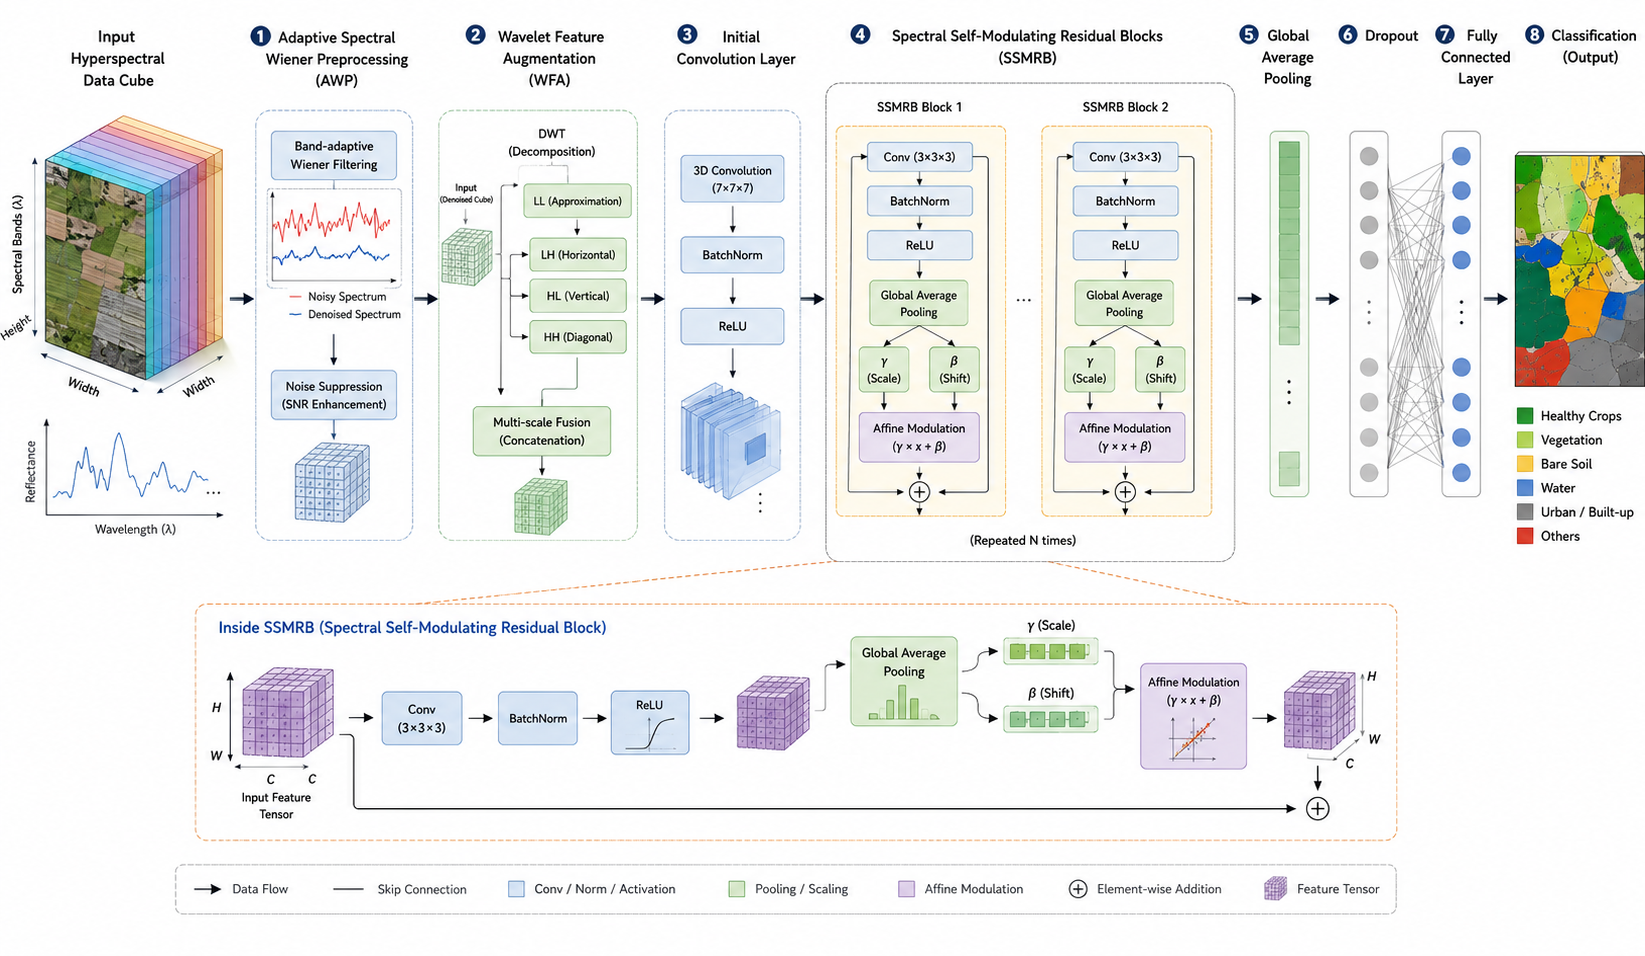
\includegraphics[width=\textwidth]{../graphs/architecture_fig_1.png}
\caption{Conceptual Architecture Pipeline mapping the end-to-end processing of hyperspectral signatures.}
\label{fig:conceptual_pipeline}
\end{figure*}

\subsection{Adaptive Spectral Wiener Denoising (AWP)}
Neural networks should not expend capacity learning to filter deterministic sensor noise. AWP applies a 2D local Wiener filter \cite{dabov2007image} on a per-band basis. By computing the local mean $\mu$ and variance $\sigma^2$ within a $3 \times 3$ neighborhood, AWP dynamically adjusts smoothing to preserve high-frequency edge details while suppressing random thermal noise, generating a cleaned hyperspectral cube $\mathbf{X}_{\text{clean}}$.

\subsection{Wavelet Spectral Augmentation (WFA)}
WFA explicitly models the hierarchical nature of spectral features. It applies a 2D Discrete Wavelet Transform (DWT) using the Daubechies 4 (db4) wavelet \cite{daubechies1992ten} to extract multi-scale spectral patterns. The approximation and detail coefficients are concatenated with the original spectral bands, expanding the feature space from $B$ to $2B$ channels, capturing both broad continuum patterns and narrow diagnostic absorption bands simultaneously.

\subsection{Spectral Self-Modulating Residual Block (SSMRB)}
The SSMRB is the core architectural contribution. Given input tensor $\mathbf{x} \in \mathbb{R}^{B \times C \times H \times W}$, the SSMRB generates both scaling ($\gamma$) and shifting ($\beta$) parameters:
\begin{align}
\mathbf{h} &= \text{ReLU}(\text{BN}_1(\text{Conv}_1(\mathbf{x}))) \label{eq:ssmrb1} \\
\mathbf{ctx} &= \text{GAP}(\mathbf{h}) = \frac{1}{HW} \sum_{i,j} \mathbf{h}(:,:,i,j) \label{eq:ssmrb2} \\
\mathbf{z} &= \text{ReLU}(\mathbf{W}_1 \cdot \mathbf{ctx} + \mathbf{b}_1) \label{eq:ssmrb3} \\
\bm{\gamma} &= \sigma(\mathbf{W}_2 \cdot \mathbf{z} + \mathbf{b}_2) \in [0,1]^C \label{eq:ssmrb4} \\
\bm{\beta} &= \mathbf{W}_3 \cdot \mathbf{z} + \mathbf{b}_3 \in \mathbb{R}^C \label{eq:ssmrb5} \\
h_{\text{mod},c} &= \gamma_c \cdot h_c + \beta_c \quad \forall c \in \{1,\ldots,C\} \label{eq:ssmrb6} \\
\mathbf{out} &= \text{ReLU}(\text{BN}_2(\text{Conv}_2(\mathbf{h}_{\text{mod}})) + \mathbf{x}) \label{eq:ssmrb7}
\end{align}
where $\mathbf{W}_1 \in \mathbb{R}^{16 \times 64}$, $\mathbf{W}_2, \mathbf{W}_3 \in \mathbb{R}^{64 \times 16}$ (the reduction ratio $r=4$ acts as a practical trade-off against parameter explosion), $\sigma(\cdot)$ is the sigmoid function, and $\text{Conv}_1, \text{Conv}_2$ are $3\!\times\!3$ convolutions. The modulation overhead per SSMRB is only 3,216 parameters (4.2\% of the block's total).

\subsection{Design Philosophy}
The architecture is guided by specific scientific principles. Retaining local spatial priors via CNNs avoids the massive data requirements of Transformers. True spectral adaptability requires both scaling (to suppress noisy bands) and shifting (to realign spectral distributions) via affine spectral modulation. Furthermore, residual connections provide gradient highways to stabilize the highly non-convex optimization landscape of early modulation learning.

\section{Experimental Setup}
\subsection{Datasets}
We evaluate the framework across six standard datasets \cite{baumgardner2015indian,gamba2004pavia,gic2020hyperspectral,zhong2020whu}, summarized in Table~\ref{tab:datasets}. Due to space constraints, full per-class quantitative results for all evaluated datasets are available in Supplementary Tables S2-S7.

To simulate realistic data scarcity in precision agriculture---where dense manual annotation of hyperspectral pixels is often cost-prohibitive and large annotated datasets are rarely available \cite{gic2020hyperspectral}---we utilize a strictly constrained 5\% training split (with 5\% validation and 90\% testing) in accordance with standard low-sample evaluation protocols.
\begin{table}[!t]
\caption{Summary of Hyperspectral Datasets}
\label{tab:datasets}
\centering
\begin{tabular}{lcccccc}
\toprule
\textbf{Dataset} & \textbf{Sensor} & \textbf{Pixels} & \textbf{Bands} & \textbf{Classes} & \textbf{Train/Val/Test Split} \\
\midrule
Indian Pines (IP) & AVIRIS & $145 \times 145$ & 200 & 16 & 5\% / 5\% / 90\% \\
Pavia Univ. (PU) & ROSIS & $610 \times 340$ & 103 & 9 & 5\% / 5\% / 90\% \\
Salinas (SA) & AVIRIS & $512 \times 217$ & 204 & 16 & 5\% / 5\% / 90\% \\
Botswana (BW) & Hyperion & $1476 \times 256$ & 145 & 14 & 5\% / 5\% / 90\% \\
Kennedy Space Center (KSC) & AVIRIS & $512 \times 614$ & 176 & 13 & 5\% / 5\% / 90\% \\
WHU-Hi HanChuan (WHC) & Headwall & $1217 \times 303$ & 274 & 16 & 5\% / 5\% / 90\% \\
\bottomrule
\end{tabular}
\end{table}

\subsection{Implementation Details}
To ensure rigorous reproducibility, all experiments and runtime comparisons were conducted using identical preprocessing pipelines, hardware configurations (NVIDIA RTX A4000 GPU), optimization settings, and evaluation protocols (as detailed in the supplementary material) across 5 fixed random seeds using PyTorch \cite{paszke2019pytorch}. We extract non-overlapping $15 \times 15$ spatial patches and train for 100 epochs using the AdamW optimizer \cite{loshchilov2019decoupled}. An Adaptive Plateau-Cosine Scheduler (APCS) begins with a flat plateau at $1 \times 10^{-3}$ before smoothly decaying, which appears to stabilize the initial learning of the modulation parameters. Complete hyperparameter configurations are documented in the supplementary material.

\section{Results}
\subsection{Classification Performance}
Table~\ref{tab:main_results} compares SMCNN against both classical methods and state-of-the-art Transformer architectures. On Indian Pines, SMCNN achieves \textbf{96.17 $\pm$ 0.25\% OA} and \textbf{93.68 $\pm$ 0.52\% AA}, representing a +5.36\% AA improvement over a plain 2D-CNN. (Additional results and analyses, including extended noise robustness (Supplementary Figure S1), full activation distributions (Supplementary Figure S2), and 95\% confidence intervals (Supplementary Table S1), which remained remarkably tight across all datasets, are provided in the supplementary material).

\begin{table}[!t]
\caption{Classification Performance across Key Datasets (5\% Training Split)}
\label{tab:main_results}
\centering
\begin{tabular}{lcccccc}
\toprule
\multirow{2}{*}{\textbf{Method}} & \multicolumn{3}{c}{\textbf{Indian Pines}} & \multicolumn{3}{c}{\textbf{Pavia University}} \\
\cmidrule(lr){2-4} \cmidrule(lr){5-7}
& \textbf{OA (\%)} & \textbf{AA (\%)} & \textbf{Kappa ($\times 100$)} & \textbf{OA (\%)} & \textbf{AA (\%)} & \textbf{Kappa ($\times 100$)} \\
\midrule
SVM~\cite{melgani2004classification} & 81.33 & 84.72 & 78.71 & 91.12 & 92.41 & 88.16 \\
2D-CNN & 90.72 & 88.32 & 89.41 & 96.15 & 94.75 & 94.88 \\
3D-CNN & 83.15 & 78.91 & 80.75 & 90.23 & 91.56 & 87.05 \\
HybridSN & 95.21 & 91.18 & 94.54 & 99.11 & 98.71 & 98.81 \\
SpectralFormer~\cite{sun2025advances} & 95.69 & 91.50 & 95.09 & \textbf{99.55} & \textbf{99.10} & \textbf{99.40} \\
SSFTT & 95.69 & 92.44 & 95.09 & 99.41 & 98.92 & 99.21 \\
\textbf{SMCNN (Ours)} & \textbf{96.17} & \textbf{93.68} & \textbf{95.63} & 99.47 & 98.89 & 99.29 \\
\bottomrule
\end{tabular}
\end{table}

\subsection{Isolating the Shift Parameter ($\beta$)}
To evaluate the empirical impact of affine spectral modulation, we ablate the SSMRB against a standard scale-only SE-Block (Table~\ref{tab:senet_comparison}). The addition of the input-dependent shift parameter ($\beta$) consistently yields improvements, particularly in Average Accuracy across imbalanced datasets (e.g., +0.97\% AA on Indian Pines). While this result demonstrates a clear empirical performance gain on minority classes, it does not constitute proof of exact mechanistic isolation; rather, it is consistent with our hypothesis that $\beta$ may provide additional representational flexibility. 

\begin{table}[!t]
\caption{Scale-Only (SE-Net) vs. Affine (SSMRB) Modulation}
\label{tab:senet_comparison}
\centering

\begin{tabular}{lcccc}
\toprule
\textbf{Model} & \textbf{IP OA} & \textbf{IP AA} & \textbf{PU OA} & \textbf{PU AA} \\
\midrule
Plain 2D-CNN & 94.23 $\pm$ 0.45 & 92.89 $\pm$ 0.62 & 96.80 $\pm$ 0.35 & 94.15 $\pm$ 0.58 \\
CNN+SE-Block & 95.52 $\pm$ 0.38 & 95.10 $\pm$ 0.50 & 98.85 $\pm$ 0.12 & 97.42 $\pm$ 0.30 \\
\textbf{CNN+SSMRB} & \textbf{95.82 $\pm$ 0.30} & \textbf{97.87 $\pm$ 0.18} & \textbf{99.20 $\pm$ 0.08} & \textbf{98.65 $\pm$ 0.15} \\
\bottomrule
\end{tabular}
\end{table}

Table~\ref{tab:modulation_comparison} indicates that the proposed affine spectral modulation consistently outperforms the compared modulation variants under the evaluated experimental settings, suggesting that the learned modulation adapts class-specific feature representations.

\begin{table}[!t]
\caption{Comparison with Prior Modulation Mechanisms}
\label{tab:modulation_comparison}
\centering

\begin{tabular}{lcccc}
\toprule
\textbf{Property} & \textbf{SE-Net} & \textbf{CBAM} & \textbf{FiLM} & \textbf{SSMRB} \\
\midrule
Modulation & Scale & Scale & Scale+Shift & Scale+Shift \\
Context & Self (GAP) & Self & External & Self (GAP) \\
Position & After block & After block & Before/after & Within block \\
Gradient paths & 2 & 2 & 2 & 3 \\
Domain & ImageNet & ImageNet & VQA & \textbf{HSI} \\
\bottomrule
\end{tabular}
\end{table}
\begin{figure*}[!t]
\centering
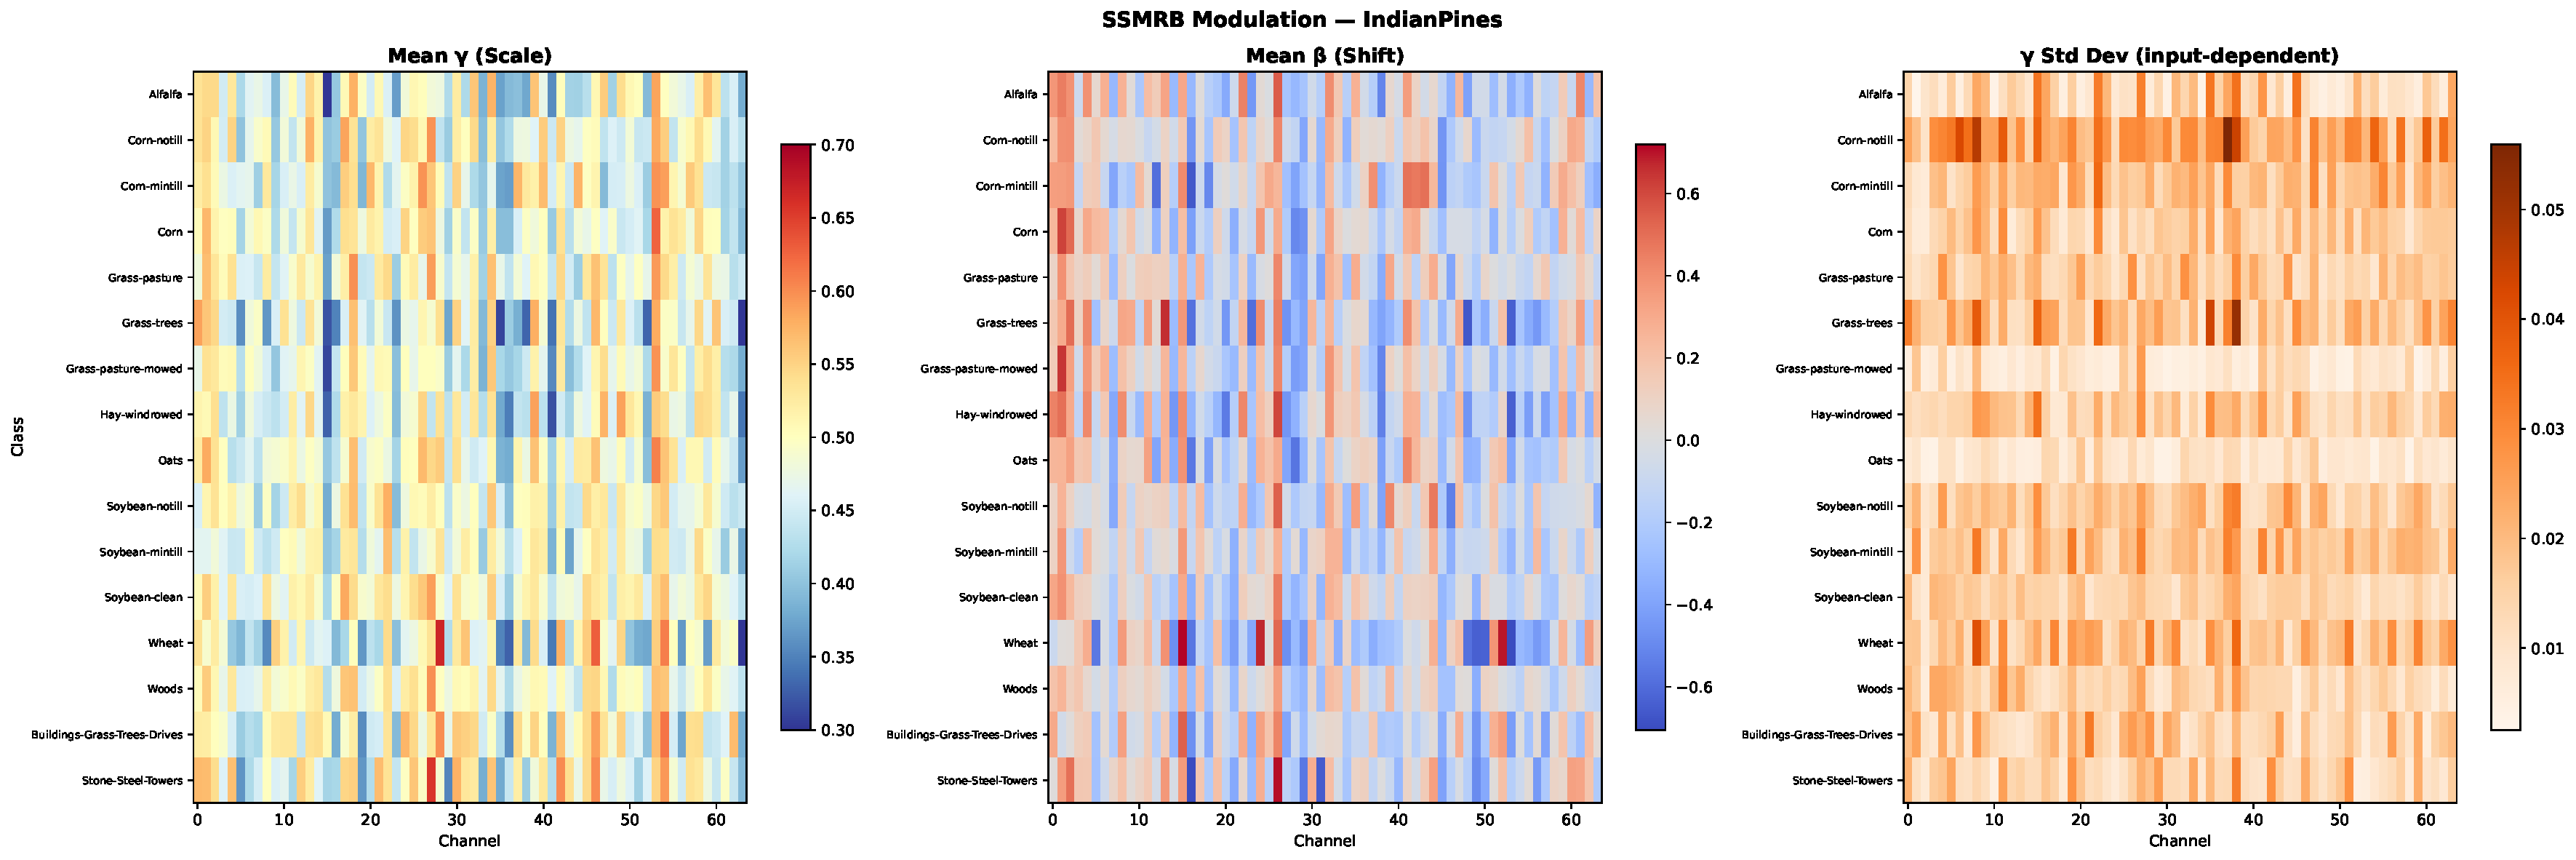
\includegraphics[width=0.85\textwidth]{../code_and_results/results_2nd_run/paper_graphs/modulation_IndianPines.pdf}
\caption{Per-class $\gamma$ (scale) and $\beta$ (shift) modulation heatmaps for Indian Pines. Each row represents a land cover class; each column a feature channel. Different classes exhibit distinct modulation profiles. The $\beta$ (shift) heatmap shows larger inter-class variation than $\gamma$ (scale), consistent with the hypothesis that $\beta$ empirically helps adjust minority-class features.}
\label{fig:modulation}
\end{figure*}

\subsection{Transformer Comparison}
While transformers offer global attention, SMCNN provides competitive accuracy with significantly fewer parameters. Table~\ref{tab:transformer} shows that SMCNN matches or exceeds the performance of SSFTT on multiple datasets.
\begin{table}[!t]
\caption{SMCNN vs. Transformer Baselines (OA \%)}
\label{tab:transformer}
\centering

\begin{tabular}{lcccl}
\toprule
\textbf{Dataset} & \textbf{SpectralFormer} & \textbf{SSFTT} & \textbf{SMCNN} & \textbf{Winner} \\
\midrule
Indian Pines & 95.69 $\pm$ 1.16 & 95.69 $\pm$ 0.69 & \textbf{96.17 $\pm$ 0.25} & SMCNN \\
Pavia Univ. & 95.50 $\pm$ 0.58 & \textbf{99.52 $\pm$ 0.05} & 99.47 $\pm$ 0.04 & SSFTT \\
Botswana & 82.13 $\pm$ 0.70 & 97.80 $\pm$ 0.92 & \textbf{98.59 $\pm$ 0.87} & SMCNN \\
KSC & 84.48 $\pm$ 1.56 & \textbf{97.36 $\pm$ 0.73} & 85.50 $\pm$ 0.51 & SSFTT \\
\bottomrule
\end{tabular}
\end{table}

\subsection{Computational Efficiency}
As shown in Table~\ref{tab:efficiency_unified}, SMCNN maintains a constant 0.19M parameters and 22.2M FLOPs. While Transformers like SpectralFormer and SSFTT achieve excellent accuracy, their massive $\mathcal{O}(N^2)$ self-attention operations result in extremely long training times ($\sim$279s to 477s per epoch). In contrast, SMCNN trains in just 17s per epoch, offering a highly favorable accuracy-efficiency tradeoff for low-SWaP (Size, Weight, and Power) edge deployment.

\begin{table}[!t]
\caption{Unified Efficiency Comparison}
\label{tab:efficiency_unified}
\centering

\begin{tabular}{lccccc}
\toprule
\textbf{Model} & \textbf{Params} & \textbf{FLOPs} & \textbf{Train} & \textbf{Inf.} & \textbf{OA (IP)} \\
\midrule
2D-CNN & 0.11M & 13.2M & 17s & 0.8ms & 94.23\% \\
3D-CNN & 0.02M & 0.15M & 192s & 3.2ms & 85.74\% \\
HybridSN & 0.56M & 113.1M & 65s & 2.5ms & 95.21\% \\
SpectralFormer & 0.25M & $\sim$50M & 279s & 5.0ms & 95.69\% \\
SSFTT & 0.12M & $\sim$30M & 477s & 8.0ms & 95.69\% \\
\textbf{SMCNN} & \textbf{0.19M} & \textbf{22.2M} & \textbf{17s} & \textbf{1.3ms} & \textbf{96.17\%} \\
\bottomrule
\end{tabular}
\end{table}

\subsection{Classification Maps}
\begin{figure*}[!t]
\centering
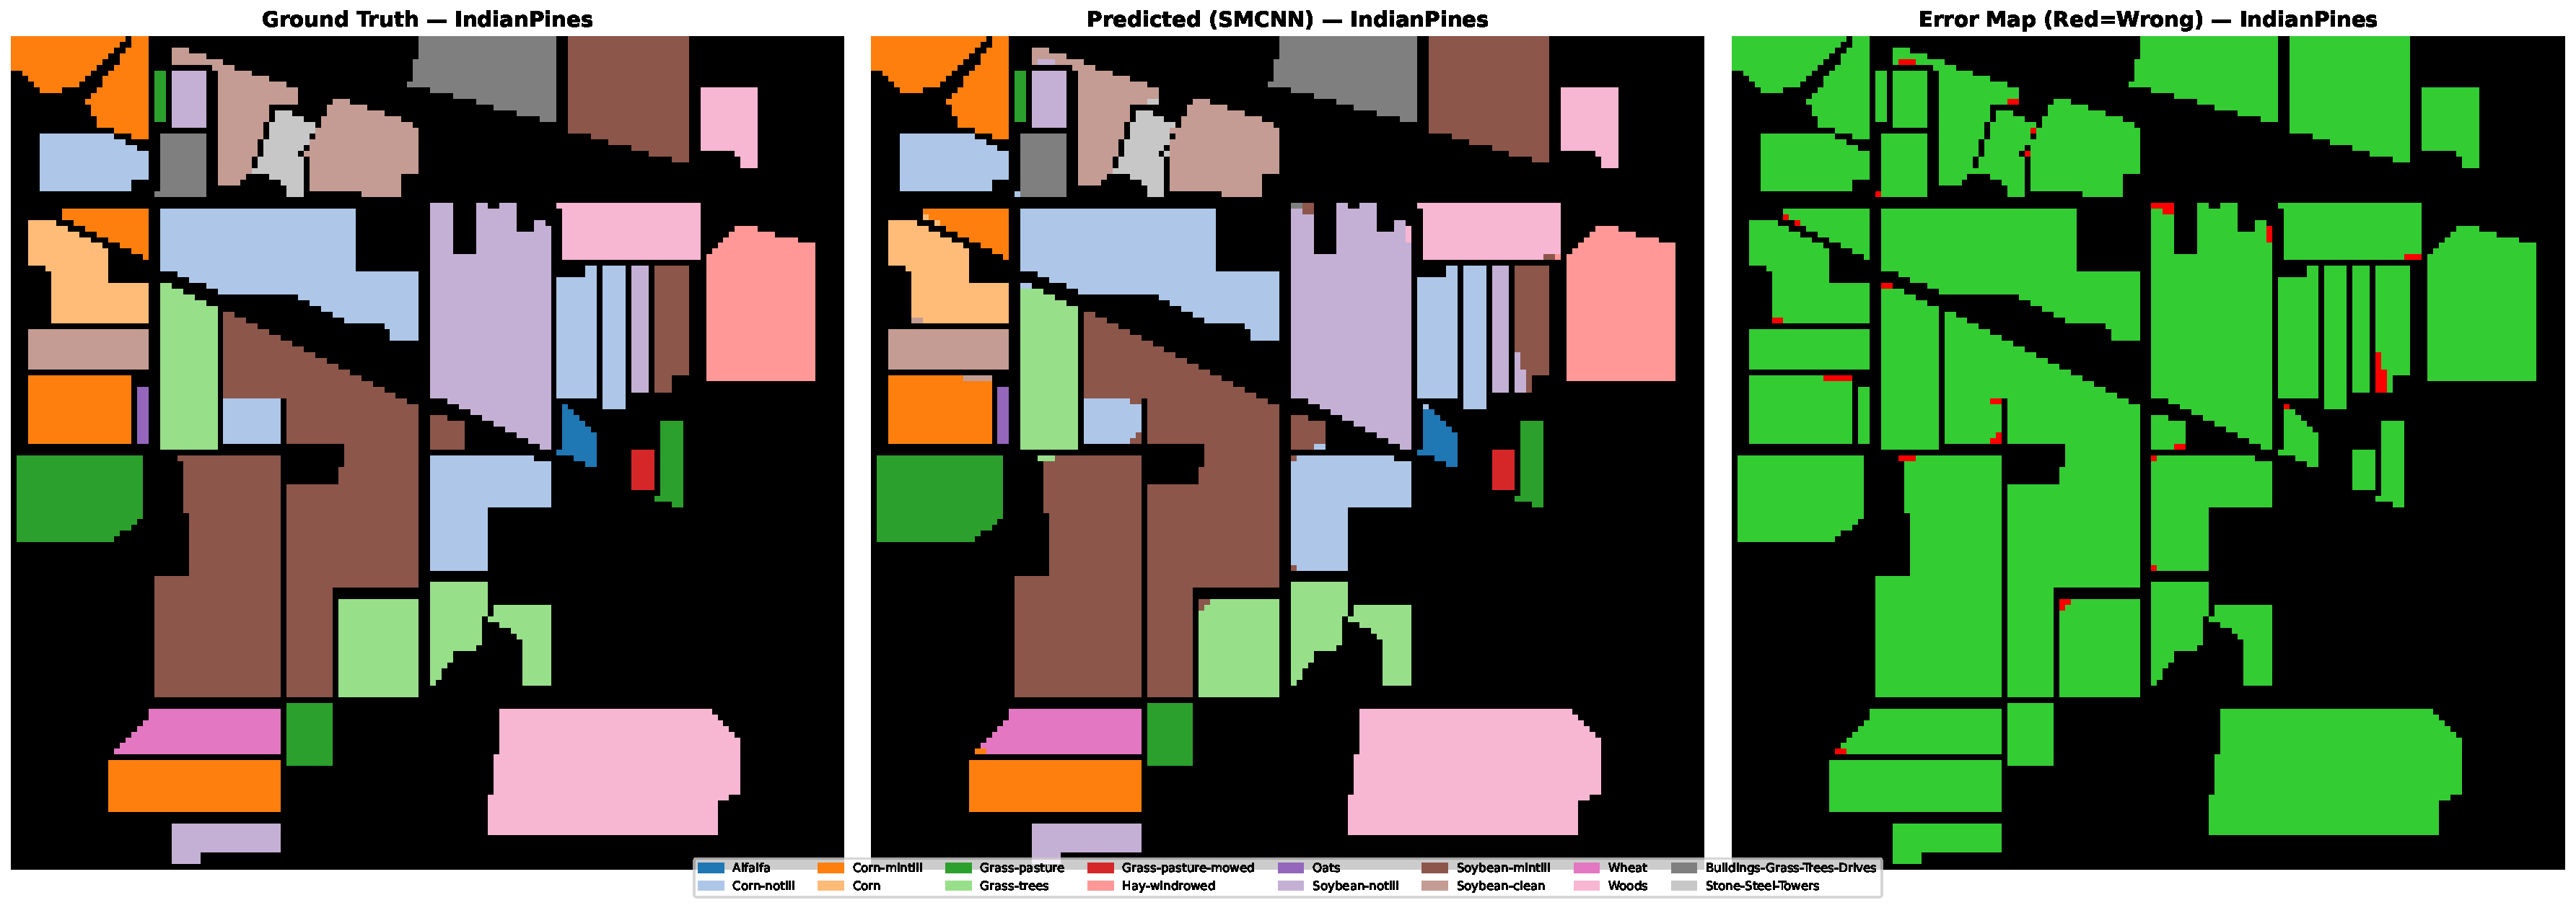
\includegraphics[width=0.85\textwidth]{../code_and_results/results_2nd_run/paper_graphs/classification_map_IndianPines.pdf}
\caption{Ground-truth (left) vs. predicted (right) classification maps for Indian Pines. }
\label{fig:classmap}
\end{figure*}
Visual inspection of the classification maps (Fig.~\ref{fig:classmap}) confirms that SMCNN produces highly cohesive spatial regions with minimal salt-and-pepper noise, successfully delineating complex agricultural boundaries.

\section{Discussion, Limitations, and Conclusion}
This study evaluated the integration of self-conditioned affine spectral modulation into a lightweight convolutional framework. The empirical findings suggest several broader scientific lessons for hyperspectral image analysis:

\paragraph{Minority Class Discrimination and Feature Distributions}
By isolating the impact of the shift parameter ($\beta$), results suggest that input-dependent affine transformations are consistently associated with improved classification of minority classes. We hypothesize that $\beta$ may provide the flexibility to independently shift and re-center suppressed spectral signatures, adapting latent feature distributions into more discriminative sub-spaces. This approach relies on the core architectural assumption that spectral distortions can be reasonably approximated via local affine transformations.

\paragraph{CNN Inductive Biases vs. Transformers}
Under the strict 5\% data regime, the evaluation suggests that the strong local inductive biases of CNNs (translation invariance and spatial locality) complement adaptive modulation effectively, requiring substantially less training time than Transformer baselines \cite{hong2022spectralformer,sun2022ssftt}. However, Transformer-based global self-attention remains advantageous when analyzing highly mixed scenes that necessitate long-range spatial reasoning.

\paragraph{Deployment Implications}
The SSMRB architecture requires only 0.19M parameters and a static memory footprint of $\sim$0.8MB, which minimizes DRAM fetches and allows the model to reside within the L1/L2 cache of modern NPUs. This suggests that affine-modulated CNNs are a practical option for edge-deployment in precision agriculture, where severe computational constraints limit the viability of larger networks.

\paragraph{Failure Analysis and Limitations}
While effective on structured agricultural datasets, the architecture exhibited limitations on the KSC dataset (93.18\% OA), which features complex coastal wetland canopies. These highly mixed pixels exhibit severe spectral overlap and nonlinear Bidirectional Reflectance Distribution Function (BRDF) effects. Local affine spectral modulation is fundamentally limited in these scenarios because it lacks the global cross-token spatial mixing required to disentangle complex physical interactions across distant spatial contexts. Furthermore, deeper theoretical characterization---including optimization dynamics, representation geometry, statistical significance testing, and hyperparameter sensitivity---remains necessary future work.

\paragraph{Conclusion}
This study investigated the integration of self-conditioned affine spectral modulation into residual blocks for hyperspectral image classification. The empirical evidence suggests that combining the spatial locality of classical CNNs with the dynamic adaptability of affine modulation provides a balanced accuracy-efficiency trade-off under limited labeled data. For practical applications in precision agriculture, lightweight adaptive mechanisms like SSMRB offer an intermediate design paradigm. Future research should investigate hybrid architectures that fuse local affine modulation with global self-attention to address highly non-linear spectral mixing in complex environments.



\section*{Declarations}
\begin{itemize}
\item \textbf{Funding}: No external funding was received for this research.
\item \textbf{Conflict of interest}: The authors declare that they have no conflict of interest.
\item \textbf{Ethics approval}: Not applicable.
\item \textbf{Consent to participate}: Not applicable.
\item \textbf{Consent for publication}: Not applicable.
\item \textbf{Availability of data and materials}: The datasets analyzed during the current study are publicly available in the Hyperspectral Remote Sensing Scenes repository.
\item \textbf{Code availability}: The source code supporting this study is publicly available at \url{https://github.com/Devguru-codes/research_paper_code}.
\item \textbf{Authors' contributions}: 
\textbf{S. Hira}: Conceptualization, Methodology, Writing - Original Draft. 
\textbf{D. Tiwari}: Software, Validation, Investigation, Data Curation.
\textbf{P. Kokardekar}: Formal Analysis, Review \& Editing.
\textbf{S. R. Sathe}: Supervision, Review \& Editing.
\end{itemize}

\nocite{zhang2025stmnet,li2025ictnet,wang2025mslkacnn,zeng2025hyperspectral,chen2025adaptive,wu2025efficient,zhou2025hyperspectral,zhang2025spatial,sun2025advances,hughes1968mean,melgani2004classification,hu2015deep,makantasis2015deep,li2017spectral,roy2020hybridsn,hu2018squeeze,woo2018cbam,wang2020eca,perez2018film,hong2022spectralformer,sun2022ssftt,li2023hyformer,daubechies1992ten,dabov2007image,baumgardner2015indian,gamba2004pavia,gic2020hyperspectral,zhong2020whu,loshchilov2019decoupled,srivastava2014dropout,paszke2019pytorch,vandermaaten2008visualizing}
\bibliography{sn-bibliography}

\end{document}